\section{Motivation}
\begin{frame}
	\frametitle{Why I use Julia}
  \begin{itemize}
    \item Fast
    \item Plays nice with shell, C/++ and Python
    \item Vectors or loops
    \item Read/Evaluate/Print/Loop (REPL)
    \item Growing ecosystem
  \end{itemize}
\end{frame}

\begin{frame}
	\frametitle{Speed}
  \begin{figure}[ht]
    \centering
    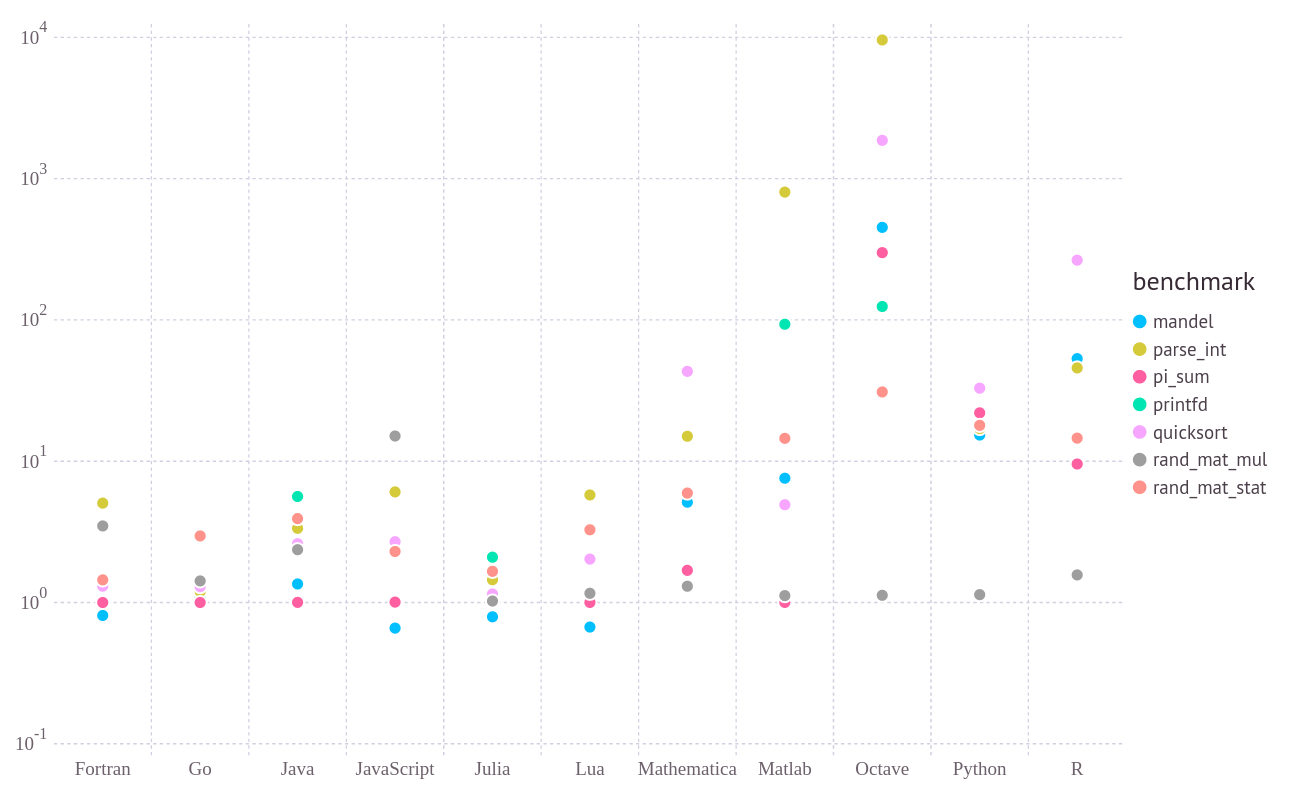
\includegraphics[width=0.8\textwidth]{benchmark}
  \end{figure}
  julialang.org
\end{frame}

\begin{frame}
	\frametitle{Calling C}
  \begin{itemize}
    \begin{small}
    \item \mint{julia}|ccall((symbol, library) or function_pointer, ReturnType,|
      \mint{julia}|(ArgumentType1, ...), ArgumentValue1, ...)|
    \item \mint{julia}|cfunction(function::Function, ReturnType::Type,|
      \mint{julia}|(ArgumentTypes...))|
    \item https://github.com/timholy/Cpp.jl
    \item https://github.com/Keno/Cxx.jl
    \end{small}
  \end{itemize}
\end{frame}

\begin{frame}[fragile]
	\frametitle{Calling C}
  \begin{tiny}
  \begin{minted}{julia}
[d9w@noise julia]$ export FOO=BAR
[d9w@noise julia]$ julia

julia> function getenv(var::AbstractString)
         val = ccall((:getenv, "libc"),
                     Cstring, (Cstring,), var)
         if val == C_NULL
           error("getenv: undefined variable: ", var)
         end
         unsafe_string(val)
       end
getenv (generic function with 1 method)

julia> getenv("FOO")
"BAR"
  \end{minted}
  \end{tiny}
\end{frame}

\begin{frame}[fragile]
	\frametitle{Cpp.jl}
  \begin{tiny}
  \begin{minted}{c}
 int timestwo(int x) {
   return 2*x;
 }

 double timestwo(double x) {
   return 2*x;
 }
  \end{minted}
  \begin{minted}{julia}
julia> x = 3.5
julia> x2 = @cpp ccall((:timestwo, libdemo), Float64, (Float64,), x)
julia> y = 3
julia> y2 = @cpp ccall((:timestwo, libdemo), Int, (Int,), y)
  \end{minted}
  \end{tiny}
\end{frame}

\begin{frame}[fragile]
	\frametitle{Cxx.jl}
  \begin{tiny}
  \begin{minted}{julia}
julia> using Cxx
julia> cxx"""#include <iostream>
       class Hello
       { 
           public:
               void hello_world(const char *now){
                   std::string snow = now;
                   std::cout << "Hello World! Now is " << snow << std::endl;
               }
        };"""
julia> hello_class = @cxxnew Hello()
julia> tstamp = string(Dates.now())
julia> @cxx hello_class -> hello_world(pointer(tstamp))
Hello World! Now is 2015-06-19T11:20:31
  \end{minted}
  \end{tiny}
\end{frame}

\begin{frame}[fragile]
	\frametitle{Calling Julia in C}
  \begin{tiny}
  \begin{minted}{c}
#include <julia.h>

int main(int argc, char *argv[])
{
    /* required: setup the Julia context */
    jl_init(NULL);

    /* run Julia commands */
    jl_eval_string("print(sqrt(2.0))");

    /* strongly recommended: notify Julia that the
         program is about to terminate. this allows
         Julia time to cleanup pending write requests
         and run all finalizers
    */
    jl_atexit_hook(0);
    return 0;
}
  \end{minted}
  \end{tiny}
\end{frame}

\begin{frame}[fragile]
	\frametitle{Calling Python}
  \begin{tiny}
  \begin{minted}{julia}
@pyimport numpy.polynomial as P
@pydef type Doubler <: P.Polynomial
    __init__(self, x=10) = (self[:x] = x)
    my_method(self, arg1::Number) = arg1 + 20
    x2.get(self) = self[:x] * 2
    x2.set!(self, new_val) = (self[:x] = new_val / 2)
end
Doubler()[:x2]
  \end{minted}
  \vspace{2.0mm}
  \begin{minted}{python}
import numpy.polynomial
class Doubler(numpy.polynomial.Polynomial):
    def __init__(self, x=10):
        self.x = x
    def my_method(self, arg1): return arg1 + 20
    @property
    def x2(self): return self.x * 2
    @x2.setter
    def x2(self, new_val):
        self.x = new_val / 2
Doubler().x2
  \end{minted}
  \end{tiny}
  \vspace{5.0mm}
  https://github.com/JuliaPy/PyCall.jl
\end{frame}

\begin{frame}[fragile]
	\frametitle{Vectors and loops}
  \begin{tiny}
  \begin{minted}{julia}
function vectorized()
    a = [1.0, 1.0]
    b = [2.0, 2.0]
    x = [NaN, NaN]

    for i in 1:1000000
        x = a + b
    end

    return
end

function devectorized()
    a = [1.0, 1.0]
    b = [2.0, 2.0]
    x = [NaN, NaN]

    for i in 1:1000000
        for index in 1:2
            x[index] = a[index] + b[index]
        end
    end

    return
end
\end{minted}
\end{tiny}
\end{frame}

\begin{frame}[fragile]
	\frametitle{Vectors and loops}
\begin{table}
\small
\begin{tabular}{*{3}{l}}
Approach & Language & Average Time \\
\hline
Vectorized & R & 0.49 \\
Devectorized & R & 4.72 \\
Vectorized & Julia & 0.24 \\
Devectorized & Julia & 0.0035 \\
\end{tabular}
\end{table}
\end{frame}

\begin{frame}[fragile]
	\frametitle{Vectors and loops}
  \begin{tiny}
  \begin{minted}{julia}
julia> X .= f.(2 .* X.^2 .+ 6 .* X.^3 .- sqrt.(X))

julia> for i in eachindex(X)
    x = X[i]
    X[i] = f(2x^2 + 6x^3 - sqrt(x))
end

julia> [1 2 3] .+ [10,20,30]
3×3 Array{Int64,2}:
 11  12  13
 21  22  23
 31  32  33

julia> s = ["The QUICK Brown", "fox     jumped", "over the LAZY dog."];

julia> s .= replace.(lowercase.(s), r"\s+", "-")
3-element Array{String,1}:
 "the-quick-brown"   
 "fox-jumped"        
 "over-the-lazy-dog."
  \end{minted}
  \end{tiny}
\end{frame}
